\documentclass[class=report, crop=false]{standalone}
\usepackage[subpreambles=true]{standalone}
\usepackage{import}

\begin{document}
The mechanical structure is based on four threaded rods to which the top and bottom plates will be attached. \\
Top and bottom plates are made from $2\text{mm}$ thick PLA (3D printed). \\
The side is made from epoxy a $1\text{mm}$ thick PLA (also 3D printed). \\
The inside structure will be based on modular discs with components that will be inserted in a desired order and quantity. \\
Each component is attached directly to the structural rods with holes in the  and nuts on the rods. \\
\newpage
For the CanSat to work as intended, the following modules are necessary (In parenthesis is their place on the satellite's render):
\begin{itemize}
\item Onboard computer (One of the dark green circular board on the render) \\
  An Arduino board, this will do all the logic needed to process and transmit the data. 
\item Sensor boards (The other dark green circurar board and the rectangular dark green board) \\
  These boards are where the sensors will be located. They will be connected to the Onboard Computer.
\item Battery component (The two light green cylinders) \\
  These will contain the batteries needed for the whole system to work properly. \\
  We are going to use two Li-Ion 18350 batteries, with capacity of $1200\text{mAh}$ each. (4.2V)
\item Mobility compartment (The dark blue servos) \\
  This compartment will include the servos used for the chambered parachute steering.
\item GPS compartment (The gray rectangular block at the top of the render) \\
  This compartment will consist of a GPS module. 
\item Ballast modules (Not pictured on the render) \\
    These modules will ensure the CanSat is stable and it is within the weight requirements.
\end{itemize}

Below we have attached a multitude of pictures and a render of the current mechanical structure. \\
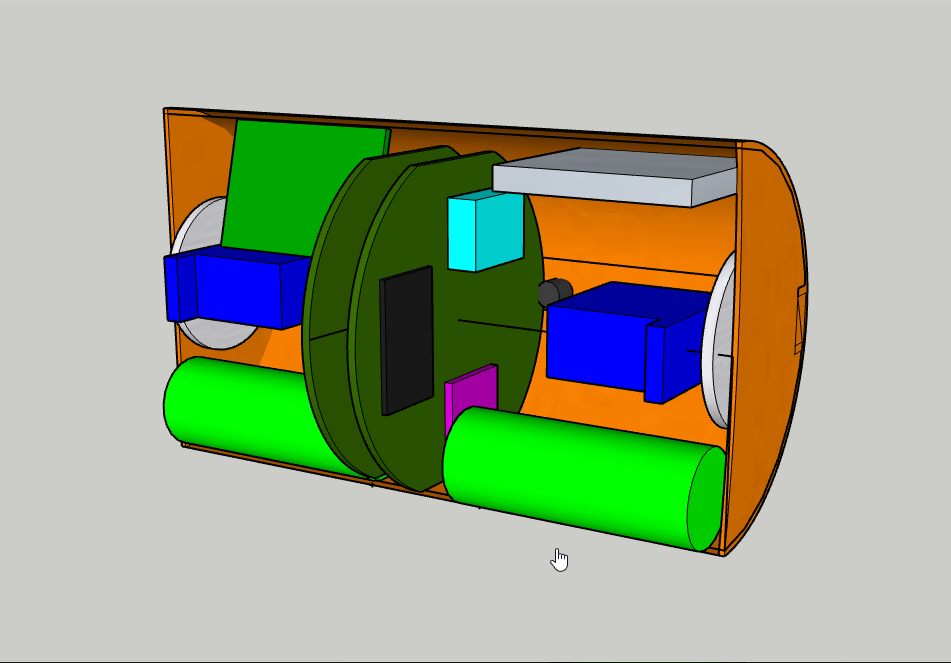
\includegraphics[width=\columnwidth]{ext/render.png}
\captionof{figure}{A render of the satellite}
\includegraphics[width=\columnwidth]{ext/fullpic.png}
\captionof{figure}{A picture of the completed satellite without the outer casing}
\end{document}
